%\chapter{Appendix}
%\label{sec:appendix}
%
%\section{Homographien bei Drehungen um ein Projektionszentrum}
%\label{sec:AppendixHomographieRotationPZ}
%
%%Homographie zwischen der Abbildungen eines Quadrates einer definierten Ausgangskamera und einer um ihr Projektionszentrum rotierten Kamera
%In diesem Beispiel werden die abgebildeten Punkte eines Quadrats einer Kamera $(C_\beta)$ mit $\beta= [\vec{b_1},\vec{b_2},\vec{b_3},C]$ in die einer anderen Kamera $(C',\beta')$ mit $\beta'= [\vec{b'_1},\vec{b'_2},\vec{b'_3},C']$  mit Hilfe einer selbst aufgestellten Homographiematrix überführt. Hierzu wird zunächst eine Szene mit den Eckpunkten des Quadrates $A_\delta, B_\delta, C_\delta, D_\delta$ und dessen Mittelpunkt mit $E_\delta$ und zwei Kameras $C_{\delta}$ und $C'_{\delta}$ definiert. Für Die Projektionszentren der Kameras gilt in hier, dass $C'_{\delta} = C_\delta$. Die Eckpunkte so wie die Kameras werden in Weltkoordinaten mit den Basen $(O,\delta)$ mit $\delta = [\vec{d_1},\vec{d_1},\vec{d_1},O]$ angegeben. Mit Hilfe der gelernten Transformationsmethoden, werden die Eckpunkte in ihre jeweiligen 2D-Bildebenenkooridnaten $(I,\tau)$ und $(I',\tau')$ umgerechnet. Nachdem die Szene vollständig definiert und die auf den Kameras abgebildeten Punkte berechnet sind, werden zwei Methoden gezeigt, mit welchem die Homographiematrix ermittelt werden kann. Da es sich in diesem Beispiel um ein selbst aufgestelltes Minimalbeispiel handelt, kommt es zu keinem überbestimmten Fall bei der der Berechnung der Homographiematrize. Da in Realbeispielen, jedoch immer damit gerechnet werden muss, dass es zu einem überbestimmten Fall kommt, wird das Verfahren, welches diesen Fall abdeckt ebenfalls aufgezeigt. Der Szenenaufbau des Minimalbeispiels soll folgendermaßen aussehen. Die Kamerakoordinatensysteme unterscheiden sich vom Weltkoordinatensystem durch eine Drehung um 180° um die \ensuremath{\vec{d}_1}-Achse. Der Ursprung beider Kamerakoordinatensysteme entspricht dem Projektionszentrum $C$. Des Weiteren ist Kamera zwei noch um $45^\circ$ um die $\vec{b_2}$ zu Kamera eins eingedreht. Es werden zwei Bilder der selben Szene mit diesen Kameras aufgenommen. Die Behauptung ist, dass sich die beiden entstandenen Bilder mit Einer Homographie ineinander überführen lassen. In Abbildung \ref{fig:Koordinatensysteme2} ist der Aufbau nochmal grafisch veranschaulicht.
%
%\begin{gather}
%	H=
%	\begin{bmatrix}
%		h_{11}&h_{12}&h_{13}\\
%		h_{21}&h_{22}&h_{23}\\
%		h_{31}&h_{32}&h_{33}
%	\end{bmatrix}
%\end{gather}\\
%
%
%\begin{minipage}{\linewidth}
%	\centering
%	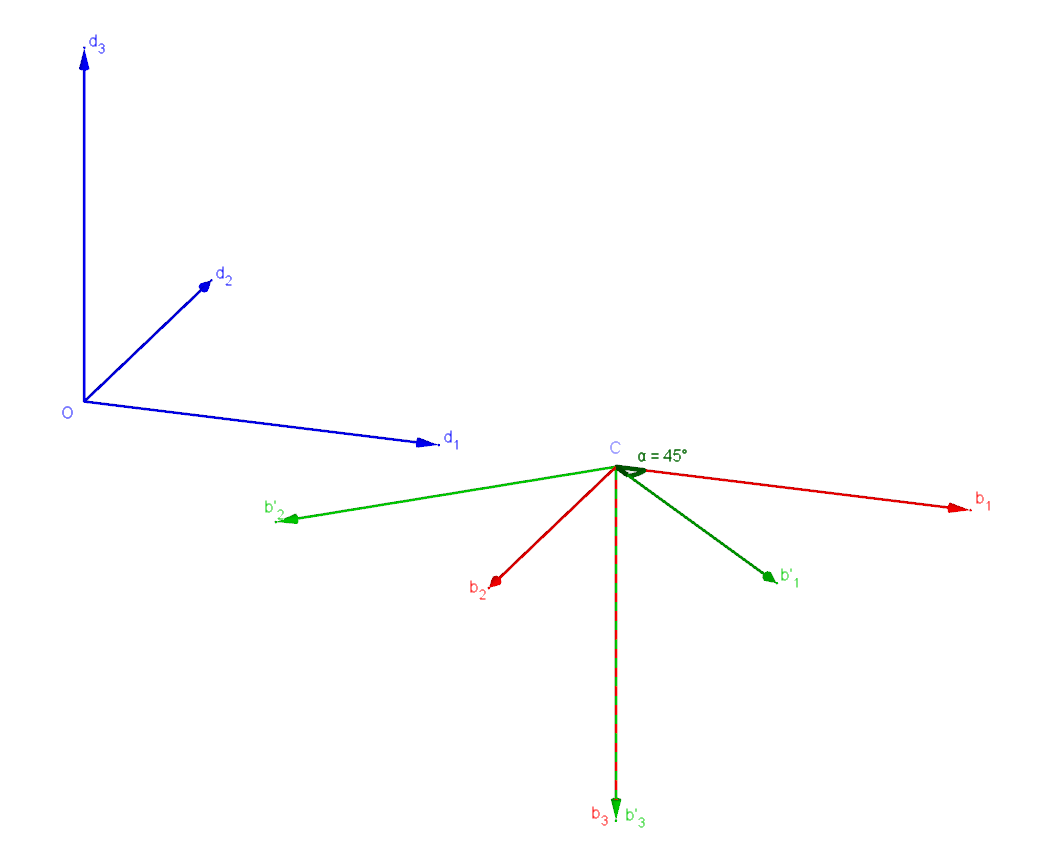
\includegraphics[width=1.\linewidth]{images/GrafikHomographieSameC.png}
%	\captionof{figure}{Weltkoordinatensystem $(O,\delta)$ mit $\delta = [\vec{d_1},\vec{d_1},\vec{d_1},O]$ und Kamerakoordinatensysteme $\beta= [\vec{b_1},\vec{b_2},\vec{b_3},C]$ und $(C',\beta')$ mit $\beta'= [\vec{b'_1},\vec{b'_2},\vec{b'_3},C']$ .}
%	\label{fig:Koordinatensysteme2}
%\end{minipage}\\ \\
%
%Als nächstes werden die intrinsischen Kameraparameter $K$ und $K'$ für beide Kameras festgelegt. Für das Beispiel
%
%\begin{gather}
%	K=K'
%	= 
%	\begin{pmatrix}
%		\zeta&0&0&0\\
%		0&\zeta&0&0\\
%		0&0&\zeta&0\\
%		0&0&1&0
%	\end{pmatrix}\\
%	\leadsto
%	\begin{pmatrix}
%		X\\Y\\Z
%	\end{pmatrix} = 
%	K
%	\begin{pmatrix}
%		X\\Y\\Z\\1
%	\end{pmatrix}
%	=
%	\begin{pmatrix}
%		\zeta X\\\zeta Y\\\zeta Z\\Z
%	\end{pmatrix}
%	=
%	\begin{pmatrix}
%		\frac{\zeta}{Z} X\\\frac{\zeta}{Z} Y\\\zeta\\1
%	\end{pmatrix}
%\end{gather}\\
%
%Für das Beispiel gilt die Bedingung, dass $\zeta \neq 0$ sein soll. Des Weiteren soll gelten, dass  \ensuremath{\vec{b}_1} gleich der Lotgeraden vom Objektpunkt zum Projektionszentrum entsptricht und somit folgt, dass \ensuremath{\vec{b}_1} in Sensorebene liegt und \ensuremath{\vec{b}_2 = \vec{b}_3 \times \vec{b}_1} ist. Der Quader besteht aus den Punkten $A_\delta,B_\delta,C_\delta, D_\delta$ und $E\delta$ in homogenen Weltkoordinaten. Die Punkte in Weltkoordinaten bekommen die Koordinatenwerte zugewiesen. 
%
%\begin{gather}
%	A_\delta=\begin{pmatrix}
%		0\\0\\2\\1
%	\end{pmatrix}, 
%	B_\delta=
%	\begin{pmatrix}
%		1\\0\\2\\1
%	\end{pmatrix},
%	C_\delta=
%	\begin{pmatrix}
%		1\\1\\2\\1
%	\end{pmatrix},
%	D_\delta=
%	\begin{pmatrix}
%		0\\1\\2\\1
%	\end{pmatrix},
%	E_\delta=
%	\begin{pmatrix}
%		\frac{1}{2}\\\frac{1}{2}\\2\\1
%	\end{pmatrix}
%\end{gather}\\
%
%Für die Transformation der Weltkoordinatentupel in die Bildebenen $I$ und $I'$ werden die Projektionsmatrizen $P=[KR|-KRC_\delta]$ und $P'=[K'R'|-K'R'C_\delta]$ aufgestellt werden. \ensuremath{R} soll eine Drehung der Punkte um 180° um die \ensuremath{\vec{d}_1}-Achse druchführen. \ensuremath{R'} muss zusätzlich im Anschluss noch eine Drehung, um \ensuremath{45^\circ} um die neue $\vec{b'_3}$-Achse von Kamera zwei, an die vorherige Drehung anhängen. Die so erhaltenen Matrizen \ensuremath{R} und \ensuremath{R'} können nun dazu verwendet werden, die Objektpunkte bezüglich des Weltkoordinatensystems $(O,\delta)$ in Punkte bezüglich der jeweiligen Kamerakoordinatensysteme $(C,\beta)$ und $(C',\beta')$ zu transformieren.
%
%
%\begin{gather}
%	\begin{bmatrix}
%		\cos(180)&-\sin(180)&0&0\\
%		\sin(180)&\cos(180)&0&0\\
%		0&0&1&0\\
%		0&0&0&1
%	\end{bmatrix}
%	\begin{pmatrix}
%		\vec{d}_1,\vec{d}_2,\vec{d}_3,O
%	\end{pmatrix}
%	=
%	\begin{bmatrix}
%		-1&0&0&0\\
%		0&-1&0&0\\
%		0&0&1&0\\
%		0&0&0&1
%	\end{bmatrix} 
%	\begin{pmatrix}
%		\vec{d}_1,\vec{d}_2,\vec{d}_3,O
%	\end{pmatrix}\\
%	\begin{bmatrix}
%		-1&0&0&0\\
%		0&-1&0&0\\
%		0&0&1&0\\
%		0&0&0&1
%	\end{bmatrix}^T =\begin{bmatrix}
%		-1&0&0&0\\
%		0&-1&0&0\\
%		0&0&1&0\\
%		0&0&0&1
%	\end{bmatrix}= R
%\end{gather}\\
%
%Im nächsten Schritt wird Kamera zwei noch um \ensuremath{45^\circ} um ihre $\vec{b'_3}$-Achse gedreht. Diese Transformation wird mit der vorherigen Transformation multipliziert und es entsteht $P'$ für Kamera zwei.
%
%\begin{gather}
%	\cos(45)=\sin(45)=\frac{1}{\sqrt{2}} = a\\
%	\begin{bmatrix}
%		a&0&a&0\\
%		0&1&0&0\\
%		-a&0&a&0\\
%		0&0&0&1
%	\end{bmatrix}
%	\begin{bmatrix}
%		-1&0&0&0\\
%		0&-1&0&0\\
%		0&0&1&0\\
%		0&0&0&1
%	\end{bmatrix}
%	=\begin{bmatrix}
%		-a&0&a&0\\
%		0&-1&0&0\\
%		a&0&a&0\\
%		0&0&0&1
%	\end{bmatrix}
%	\begin{pmatrix}
%		\vec{d}_1,\vec{d}_2,\vec{d}_3,O
%	\end{pmatrix}\\
%	=\begin{bmatrix}
%		-a&0&a&0\\
%		0&-1&0&0\\
%		a&0&a&0\\
%		0&0&0&1
%	\end{bmatrix}^T
%	=
%	\begin{bmatrix}
%		-a&0&a&0\\
%		0&-1&0&0\\
%		a&0&a&0\\
%		0&0&0&1
%	\end{bmatrix}
%	= R'
%\end{gather}\\
%
%Handelt es sich bei den Kamerakoordinatensystemen nicht um karteische Koordinatensysteme, so muss von den Rotationsmatrizen jeweils die Inverse genommen werden, um \ensuremath{R} und \ensuremath{R'} zu erhalten. Die Inversen Rotationsmatrizen werden in den folgenden Gleichungen nicht mit $R^{-1}$, sondern $R$ bezeichnet. So entsprechen sie auch den Notationen der Literatur\cite{Elements,HZ}. Sind die Matrizen \ensuremath{R} und \ensuremath{R'} ermittelt, können nun die Punkte des Quadrats im Raum in Punkte der jeweiligen Kameras umgerechnet werden. Für Punkte spezifisch Kamera eins ergeben sich die in den Gleichungen 3.23 bis 3.27 aufgezeigten Werte.
%
%
%\begin{gather}
%	\begin{pmatrix}
%		A_\beta\\1
%	\end{pmatrix}
%	=
%	\begin{bmatrix}
%		-1&0&0&0\\
%		0&-1&0&0\\
%		0&0&1&0\\
%		0&0&0&1
%	\end{bmatrix}
%	\begin{pmatrix}
%		0\\0\\2\\1
%	\end{pmatrix}
%	=
%	\begin{pmatrix}
%		0\\0\\2\\1
%	\end{pmatrix}\\
%	\begin{pmatrix}
%		B_\beta\\1
%	\end{pmatrix}
%	=
%	\begin{bmatrix}
%		-1&0&0&0\\
%		0&-1&0&0\\
%		0&0&1&0\\
%		0&0&0&1
%	\end{bmatrix}
%	\begin{pmatrix}
%		1\\0\\2\\1
%	\end{pmatrix}
%	=
%	\begin{pmatrix}
%		-1\\0\\2\\1
%	\end{pmatrix}\\
%	\begin{pmatrix}
%		C_\beta\\1
%	\end{pmatrix}
%	=
%	\begin{bmatrix}
%		-1&0&0&0\\
%		0&-1&0&0\\
%		0&0&1&0\\
%		0&0&0&1
%	\end{bmatrix}
%	\begin{pmatrix}
%		1\\1\\2\\1
%	\end{pmatrix}
%	=
%	\begin{pmatrix}
%		-1\\-1\\2\\1
%	\end{pmatrix}\\
%	\begin{pmatrix}
%		D_\beta\\1
%	\end{pmatrix}
%	=
%	\begin{bmatrix}
%		-1&0&0&0\\
%		0&-1&0&0\\
%		0&0&1&0\\
%		0&0&0&1
%	\end{bmatrix}
%	\begin{pmatrix}
%		0\\1\\2\\1
%	\end{pmatrix}
%	=
%	\begin{pmatrix}
%		0\\-1\\2\\1
%	\end{pmatrix}\\
%	\begin{pmatrix}
%		E_\beta\\1
%	\end{pmatrix}
%	=
%	\begin{bmatrix}
%		-1&0&0&0\\
%		0&-1&0&0\\
%		0&0&1&0\\
%		0&0&0&1
%	\end{bmatrix}
%	\begin{pmatrix}
%		\frac{1}{2}\\\frac{1}{2}\\2\\1
%	\end{pmatrix}
%	=
%	\begin{pmatrix}
%		-\frac{1}{2}\\-\frac{1}{2}\\2\\1
%	\end{pmatrix}
%\end{gather}
%
%Für Punkte spezifisch Kamera zwei ergeben sich die Punkte aus den Gleichungen 3.28 bis 3.32.
%
%\begin{gather}
%	\begin{pmatrix}
%		A'_{\beta'}\\1
%	\end{pmatrix}
%	=
%	\begin{bmatrix}
%		-a&0&a&0\\
%		0&-1&0&0\\
%		a&0&a&0\\
%		0&0&0&1
%	\end{bmatrix}
%	\begin{pmatrix}
%		0\\0\\2\\1
%	\end{pmatrix}
%	=
%	\begin{pmatrix}
%		2a\\0\\2a\\1
%	\end{pmatrix}\\
%	\begin{pmatrix}
%		B'_{\beta'}\\1
%	\end{pmatrix}
%	=
%	\begin{bmatrix}
%		-a&0&a&0\\
%		0&-1&0&0\\
%		a&0&a&0\\
%		0&0&0&1
%	\end{bmatrix}
%	\begin{pmatrix}
%		1\\0\\2\\1
%	\end{pmatrix}
%	=
%	\begin{pmatrix}
%		a\\0\\3a\\1
%	\end{pmatrix}\\
%	\begin{pmatrix}
%		C'_{\beta'}\\1
%	\end{pmatrix}
%	=
%	\begin{bmatrix}
%		-a&0&a&0\\
%		0&-1&0&0\\
%		a&0&a&0\\
%		0&0&0&1
%	\end{bmatrix}
%	\begin{pmatrix}
%		1\\1\\2\\1
%	\end{pmatrix}
%	=
%	\begin{pmatrix}
%		a\\-1\\3a\\1
%	\end{pmatrix}\\
%	\begin{pmatrix}
%		D'_{\beta'}\\1
%	\end{pmatrix}
%	=
%	\begin{bmatrix}
%		-a&0&a&0\\
%		0&-1&0&0\\
%		a&0&a&0\\
%		0&0&0&1
%	\end{bmatrix}
%	\begin{pmatrix}
%		0\\1\\2\\1
%	\end{pmatrix}
%	=
%	\begin{pmatrix}
%		2a\\-1\\2a\\1
%	\end{pmatrix}\\
%	\begin{pmatrix}
%		E'_{\beta'}\\1
%	\end{pmatrix}
%	=
%	\begin{bmatrix}
%		-a&0&a&0\\
%		0&-1&0&0\\
%		a&0&a&0\\
%		0&0&0&1
%	\end{bmatrix}
%	\begin{pmatrix}
%		\frac{1}{2}\\\frac{1}{2}\\2\\1
%	\end{pmatrix}
%	=
%	\begin{pmatrix}
%		\frac{3}{2}a\\-\frac{1}{2}\\\frac{5}{2}a\\1
%	\end{pmatrix}
%\end{gather}\\
%
%Die entstandenen Punkte sind nun entsprechend der Kamerakoordinatensysteme definiert. Jetzt müssen noch die jeweiligen Kameramatrizen $K$ und $K'$ mit diesen verrechnet werden, um so die 2D-Bildebenenpunkte der entsprechenden Kameras zu erhalten. $\zeta$ bekommt in diesem Beispiel den Wert -1, das bedeutet laut der Definition der Kamerakoordinatensysteme, dass der Sensor sich hinter dem Projektionszentrum befindet. Das entstehende Bild ist somit um \ensuremath{180^\circ} gedreht auf dem Sensor abgebildet.
%
%\begin{gather}
%	K =	K'=
%	\begin{pmatrix}
%		\zeta&0&0&0\\
%		0&\zeta&0&0\\
%		0&0&\zeta&0\\
%		0&0&1&0
%	\end{pmatrix}=
%	\begin{pmatrix}
%		-1&0&0&0\\
%		0&-1&0&0\\
%		0&0&-1&0\\
%		0&0&1&0
%	\end{pmatrix}
%\end{gather}
%
%Man kann natürlich wie bereits gewohnt die Rotationsmatrizen und die Kameramatrizen bereits im Vorhinein miteinander multiplizieren und dann auf einen 3D-Weltpunkt anwenden. Auf diese Weise bekommt man die fertigen Projektionsmatrizen  $P=[KR|-KRC_\delta]$ und $P'=[K'R'|-K'R'C_\delta]$. In diesem Beispiel werden sie nochmal getrennt voneinander auf die Punkte angewandt. Die fünf Punkte werden jeweils in einer Matrix zusammengeschrieben und mit $K$ beziehungsweise $K'$ verrechnet. 
%
%\begin{gather}
%	K \cdot 
%	\begin{pmatrix}
%		0&-1&-1&0&-\frac{1}{2}\\
%		0&0&-1&-1&-\frac{1}{2}\\
%		2&2&2&2&2\\
%		1&1&1&1&1
%	\end{pmatrix}=
%	\begin{pmatrix}
%		-1&0&0&0\\
%		0&-1&0&0\\
%		0&0&-1&0\\
%		0&0&1&0
%	\end{pmatrix}
%	\begin{pmatrix}
%		0&-1&-1&0&-\frac{1}{2}\\
%		0&0&-1&-1&-\frac{1}{2}\\
%		2&2&2&2&2\\
%		1&1&1&1&1
%	\end{pmatrix}\\=
%	\begin{pmatrix}
%		0&1&1&0&-\frac{1}{2}\\
%		0&0&1&1&-\frac{1}{2}\\
%		-2&-2&-2&-2&-2\\
%		2&2&2&2&2
%	\end{pmatrix}\\
%	\simeq
%	\begin{pmatrix}
%		0&\frac{1}{2}&\frac{1}{2}&0&\frac{1}{4}\\
%		0&0&\frac{1}{2}&\frac{1}{2}&\frac{1}{4}\\
%		-1&-1&-1&-1&-1\\
%		1&1&1&1&1
%	\end{pmatrix}	
%	\simeq
%	\begin{pmatrix}
%		0&\frac{1}{2}&\frac{1}{2}&0&\frac{1}{4}\\
%		0&0&\frac{1}{2}&\frac{1}{2}&\frac{1}{4}\\
%		1&1&1&1&1
%	\end{pmatrix}\\
%	K' \cdot 	\begin{pmatrix}
%		2a&a&a&2a&\frac{3}{2}a\\
%		0&0&-1&-1&-\frac{1}{2}\\
%		2a&3a&3a&2a&\frac{5}{2}a\\
%		1&1&1&1&1
%	\end{pmatrix}=
%	\begin{pmatrix}
%		-1&0&0&0\\
%		0&-1&0&0\\
%		0&0&-1&0\\
%		0&0&1&0
%	\end{pmatrix}
%	\begin{pmatrix}
%		2a&a&a&2a&\frac{3}{2}a\\
%		0&0&-1&-1&-\frac{1}{2}\\
%		2a&3a&3a&2a&\frac{5}{2}a\\
%		1&1&1&1&1
%	\end{pmatrix}\\=
%	\begin{pmatrix}
%		-2a&-a&-a&-2a&-\frac{3}{2}a\\
%		0&0&1&1&\frac{1}{2}\\
%		-2a&-3a&-3a&-2a&-\frac{5}{2}a\\
%		2a&3a&3a&2a&\frac{5}{2}a
%	\end{pmatrix}\\
%	\simeq
%	\begin{pmatrix}
%		-1&-\frac{1}{3}&-\frac{1}{3}&-1&\frac{3}{5}\\
%		0&0&\frac{1}{3a}&\frac{1}{2a}&\frac{1}{5}a\\
%		-1&-1&-1&-1&-1\\
%		1&1&1&1&1
%	\end{pmatrix}
%	\simeq
%	\begin{pmatrix}
%		-1&-\frac{1}{3}&-\frac{1}{3}&-1&\frac{3}{5}\\
%		0&0&\frac{1}{3a}&\frac{1}{2a}&\frac{1}{5a}\\
%		1&1&1&1&1
%	\end{pmatrix}
%\end{gather}\\
%
%Die Entstandenen Punkte beider Kameras ergeben die in Abblidung \ref{ErgebniseHomographie1} veranschaulichten Abblildungen, des Quadrats mit seinem Mittelpunkt, auf den jeweiligen Kamerabildebenen. Die aus den Objektpunkten $M_\delta$ entstandenen 2-D-Bildebenenkoordinaten $m_\tau$ und $m'_{\tau'}$ werden in den Koordinatensystemen $(I,\tau)$ mit $(\tau = \vec{b_1},\vec{b_2},\vec{b_4})$ und $(I',\tau')$ mit $(\tau = \vec{b'_1},\vec{b'_2},\vec{b'_4})$ dargestellt.\\
%
%\begin{minipage}{\linewidth}
%	\centering
%	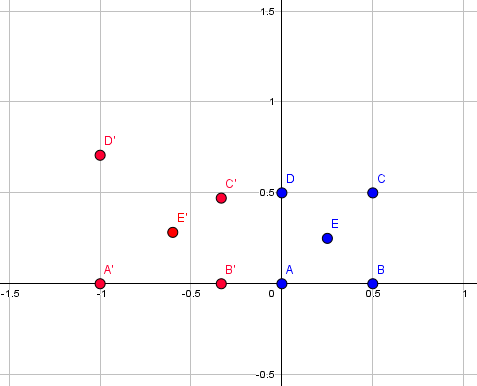
\includegraphics[width=0.8\linewidth]{images/Geogebra.png}
%	\captionof{figure}{in blau ist die Abblidung des Quaders von Kamera eins und in rot die Abbildung des selben Quaders in Kamera zwei}
%	\label{ErgebniseHomographie1}
%\end{minipage}\\ \\
%
%Die fertigen Bildebenenkoordinaten beider Kameras, sollen nun durch eine eigens aufgestellte Homographiematrix $H$ ineinander überführt werden. Um eine Homographiematrix mit 
%$H=
%\begin{bmatrix}
%h_{11}&h_{12}&h_{13}\\
%h_{21}&h_{22}&h_{23}\\
%h_{31}&h_{32}&h_{33}
%\end{bmatrix}
%$ zu erhalten werden die Punkte beider Kameras in eine Koeffizientenmatrix eingetragen, welche sich nach dem in den Gleichungen 4.40 bis 3.52 laufenden Schema ergibt. Das Verfahren wird anhand der Bildebenekoordinagen aufgezeigt.
%
%\begin{gather}
%	H\cdot m_\tau = m'_{\tau}\\
%	\begin{bmatrix}
%		h_{11}&h_{12}&h_{13}\\
%		h_{21}&h_{22}&h_{23}\\
%		h_{31}&h_{32}&h_{33}
%	\end{bmatrix}
%	\cdot
%	\begin{bmatrix}
%		\\m_\tau\\\\
%	\end{bmatrix}
%	=
%	\begin{bmatrix}
%		\\m'_{\tau'}\\\\
%	\end{bmatrix}\\
%	\begin{bmatrix}
%		h_{11}&h_{12}&h_{13}\\
%		h_{21}&h_{22}&h_{23}\\
%		h_{31}&h_{32}&h_{33}
%	\end{bmatrix}
%	\cdot
%	\begin{bmatrix}
%		x\\y\\z
%	\end{bmatrix}
%	=
%	\begin{bmatrix}
%		x'\\y'\\z'
%	\end{bmatrix}
%\end{gather}
%
%Aus Gleichung 3.42 lassen sich ein Gleichungssystem mit zwölf Bekannten und neun unbekannten aufstellen.  
%
%\begin{gather}
%	h_{11}x+h_{12}y+h_{13}z= \lambda x'\\
%	h_{21}x+h_{22}y+h_{23}z= \lambda y'\\
%	h_{31}x+h_{32}y+h_{33}z= \lambda z'
%\end{gather}
%
%Da mit homogenen Koordinaten gearbeitet wird und somit $z$ und $z'$ = 1 sind, ergibt sich für die letzte Zeile $h_{31}x+h_{32}y+h_{33}z= 1$. Dieser Ausdruck kann in den ersten beiden Gleichungen für $\lambda$ eingesetzt werden. Pro Punktepaar $m_\tau$ und $m'_{\tau'}$ ergeben sich somit zwei Gleichungen. 
%
%\begin{gather}
%	h_{11}x+h_{12}y+h_{13}z= (h_{31}x+h_{32}y+h_{33}z) \cdot x'\\
%	h_{21}x+h_{22}y+h_{23}z= (h_{31}x+h_{32}y+h_{33}z) \cdot y'
%\end{gather}
%
%Für den Aufbau der nötigen Koeffizientenmatrix werden beide Ausdrücke noch nach Null aufgelöst, so dass sich die Gleichungen 3.48 und 3.49 aus 3.46 und 3.47 ergeben.
%
%\begin{gather}
%	h_{11}x+h_{12}y+h_{13}z -(h_{31}x+h_{32}y+h_{33}z) \cdot x'= 0 \\	h_{21}x+h_{22}y+h_{23}z-(h_{31}x+h_{32}y+h_{33}z) \cdot y'=0
%\end{gather}
%\begin{gather}
%	\leadsto h_{11}x+h_{12}y+h_{13}z -h_{31}x\cdot x' - h_{32}y \cdot x'-h_{33}z\cdot x'= 0\\
%	\leadsto h_{21}x+h_{22}y+h_{23}z-h_{31}x\cdot y -h_{32}y \cdot y -h_{33}z) \cdot y'=0
%\end{gather}
%
%Die enstandnen Gleichungen werden jetzt pro Punktepaar $m_\tau$ und $m'_{\tau'}$ in eine Matrix nach folgendem Schema eingetragen.\cite{Elements,HZ,Schwarz,Heipke}
%
%\begin{gather}
%	\begin{pmatrix}
%		x_1&y_1&1&0&0&0&x_1 x'_1&y_1 x'_1 & 1\cdot x'_1\\
%		0&0&0&x_1&y_1&1&x_1 y'_1&y_1 y'_1 & 1\cdot y'_1\\
%		&&&&&.&&&\\	
%		&&&&&.&&&\\	
%		&&&&&.&&&\\	
%		x_i&y_i&1&0&0&0&x_i x'_i&y_i x'_i & 1\cdot x'_i\\
%		0&0&0&x_i&y_i&1&x_i y'_i&y_i y'_i & 1\cdot y'_i
%	\end{pmatrix}
%	\cdot
%	\begin{pmatrix}
%		h1\\h2\\.\\.\\.\\hi
%	\end{pmatrix}
%	=0
%\end{gather}
%
%Wenn ein nicht überbestimmter Fall vorliegt, sprich wenn der Rang der Koeffizientenmatrix genau acht und nicht höher beträgt, kann aus der Koeffizientenmatrix einfach der Nullraum berechnet werden, um so die Einträge für die 3x3-Homographiematrix zu erhalten\cite{HZ,Elements,Schwarz}. Gesucht wird also ein Vector $\vec{x}$, für den gilt das $H \cdot x = 0$. Der gesuchte Vektor $\vec{x}$ entspricht dem Kern der Koeffizientenmatrix und ist ein Spaltenvektor mit 9 Einträgen, welche in die 3x3-Homographiematrix eingetragen werden können\cite{HZ,Schwarz}. Tritt nun der Fall ein, dass es zu einem überbestimmtes System kommt, \textcolor{red}{was Beipielsweise auftritt wenn mehr als neun Punktepaare durch eine Homographie ineinander überführt werden sollen}, so kann nicht mehr die Ermittlung des Nullraums für die Berechnung der Homographiematrix genutzt werden. Für die Lösung überbestimmter Gleichungssysteme bietet sich die Singulärwertzerlegung an\cite{HZ}\cite{Scholz}. Das bedeutet es wird nicht derjenige Vektor $\vec{x}$ gesucht für den gilt $H \cdot x = 0$, sondern es wird derjenige Vektor $\vec{x}$ gesucht, für den \ensuremath{\parallel H \cdot x\parallel} minimal wird\cite{HZ,Schwarz}. Die Singulärwertzerlegung von zum Beispiel der Koeffizientenmatrix ist eine Faktorisierung einer beliebeigen Matrix \ensuremath{A \in \mathbb{R}^{mxn}} der Form \ensuremath{A = U \cdot S \cdot V^T} mit orthogonalen Matrizen \ensuremath{U \in \mathbb{R}^{m \times n}} und \ensuremath{V \in \mathbb{R}^{m \times n}} sowie mit einer Diagonalmatrix. 
%
%\begin{gather}
%	S = \begin{pmatrix}
%		s_1&&...&&0&0&&...&&0\\
%		.&.&&&.&.&&&&.\\
%		.&&.&&.&.&&&&.\\
%		.&&&.&.&.&&&&.\\
%		0&&...&&s_r&0&&...&&0\\	
%		0&&...&&0&0&&...&&0\\
%		.&&&&.&.&&&&.\\
%		.&&&&.&.&&&&.\\	
%		.&&&&.&.&&&&.\\	
%		0&&...&&0&0&&...&&0\\	
%	\end{pmatrix}
%\end{gather}
%
%Dabei soll für die Singulärwerte $s_1$ bis $s_r$ gelten, dass \ensuremath{s_1 \geq s_2 \geq ... \geq s_r \ge 0 }\cite{Scholz}. Entsprechend dieser Methode wird eine Singulärwertszerlegung, kurz $SVD$ der entstandenen Koeffizientenmatrix durchgeführt. Wir erhalten 3 Matrizen $U \cdot S\cdot V^T$. Durch die Zerlegung sind die diagonaleinträge von $S$ in einer absteigenden Reihenfolge sortiert. Die Spalte von $V^T$, welche mit dem kleinsten Singulärwert von $S$ korrespondiert, ergibt den Vektor $\vec{x}$, für den \ensuremath{\parallel H \cdot x\parallel} minimal wird. Somit gleichen die neun Einträge der Homographiematrix gleich der letzten Spalte von $V$. Das Ergebnis für $H$ hat dann die folgende Form
%
%\begin{gather}
%	H=
%	\begin{pmatrix}
%		v_{19}&v_{29}&v_{39}\\
%		v_{49}&v_{59}&v_{69}\\
%		v_{79}&v_{89}&v_{99}
%	\end{pmatrix}
%\end{gather}
%
%Für das Minimalbeispiel mit reinen Punkten, welches in diesem Kapitel erstellt wurde, würde die Herleitung der Homographiematrix über die Ermittlung des Nullraumes der Koeffizientenmatrix genügen. Für die Matrix $H$ ergibt sich aus den Werten der im Beispiel verwendeten Punkte
%
%\begin{gather}
%	\begin{pmatrix}
%		1&0&-1\\
%		0&\sqrt{2}&0\\
%		1&0&1
%	\end{pmatrix}
%\end{gather}
%
%Nun werden die Punkte aus Kamera eins s mit Hilfe von $H$ in die Punkte von Kamera zwei überführt und umgekehrt werden die Punkte aus Kamera zwei mit der Inversen $H^{-1}$ in die Punkte von Kamera eins überführt. 
%
%\begin{gather}
%	x'=H \cdot x \leadsto 
%	\begin{pmatrix}
%		-1&-\frac{1}{3}&-\frac{1}{3}&-1\\
%		0&0&\frac{1}{3a}&\frac{1}{2a}\\
%		1&1&1&1
%	\end{pmatrix}= 	\begin{pmatrix}
%		1&0&-1\\
%		0&\sqrt{2}&0\\
%		1&0&1
%	\end{pmatrix}
%	\cdot
%	\begin{pmatrix}
%		0&\frac{1}{2}&\frac{1}{2}&0\\
%		0&0&\frac{1}{2}&\frac{1}{2}\\
%		1&1&1&1
%	\end{pmatrix}\\
%	x=H^{-1} \cdot x' \leadsto 
%	\begin{pmatrix}
%		0&\frac{1}{2}&\frac{1}{2}&0\\
%		0&0&\frac{1}{2}&\frac{1}{2}\\
%		1&1&1&1
%	\end{pmatrix}
%	= 	\begin{pmatrix}
%		\frac{1}{2}&0&\frac{1}{2}\\
%		0&\frac{1}{\sqrt{2}}&0\\
%		\frac{1}{2}&0&\frac{1}{2}
%	\end{pmatrix}
%	\cdot
%	\begin{pmatrix}
%		-1&-\frac{1}{3}&-\frac{1}{3}&-1\\
%		0&0&\frac{1}{3a}&\frac{1}{2a}\\
%		1&1&1&1
%	\end{pmatrix}
%\end{gather}
%
%
%\section{Realbeispiel der Homographieberechnung bei Drehung um einen Drehpunkt}
%\label{sec:AppendixHomographieRotationDP}
%
%
%
%Im folgenden wird das breits bekannte Beipiel für die Drehung um das Projektionszentrum, für die Drehung um einen Drehpunkt umgebaut. Danach soll nach dem gleichen Verfahren wie im vorherignen Beispiel aufgezeigt wurde eine Homographiematrix ermittelt werden, welche die Bildebenenkoordinaten der einen Kamera in die der anderen Kamera überführen kann. Die Herangehensweise für  dieses Beispiel größtenteils die selbe wie in dem Beispiel zuvor.Der unterschied liegt lediglich in der Transformation der Punkte in as Koordinatensystem von der gedrehten Kamera zwei. Diese besteht, im Gegensatzt zum vorherigen Beispiel, nicht nur aus hintereinander geschalteten Rotationen, sondern beinhlatet des Weiteren noch zwei Translationen. Die komplette Transformationsmatrix wird, um der vorherigen Notation gerecht zu bleiben, wieder mit $R$ beziehungsweise $R'$ notiert, auch wenn es sich hier nicht mehr um eine Reine Rotation handelt. In der Literatur wird die gesamte Transformationsmatrix ebenfalls mit $R$ notiert\cite{HZ,Elements,Schwarz}. $R$ und $R'$ bestehen aus insgesamt drei Transformationsmatrizen \ensuremath{R = \text{Verschiebung}_1 \cdot \text{Rotation} \cdot \text{Verschiebung}_2}. Da die Position des Projektionszentrums von Kamera zwei nicht mehr mit dem von Kamera eins übereinstimmt, muss diese erst mit Hilfe einer Tranformationsmatrix $T$ berechnet werden. $C_{\delta} = [0 \;0 \;0\; 1]$ sind die Koordinaten von Kamera eins in Weltkoordinaten. Da in diesem Beispiel das Kamerakoodrinatensystem von Kamera eins und das Weltkoordinatensystem deckungsgleich sind heißt das,  $C_{\beta} = [0 \;0 \;0\; 1]$. somit ist Matrix $R$, welche die Transformation der ersten Kamera im Bezug auf das Weltkoordinatensystem beschreibt gleich der Einheitsmatrix.
%
%\begin{minipage}{\linewidth}
%	\centering
%	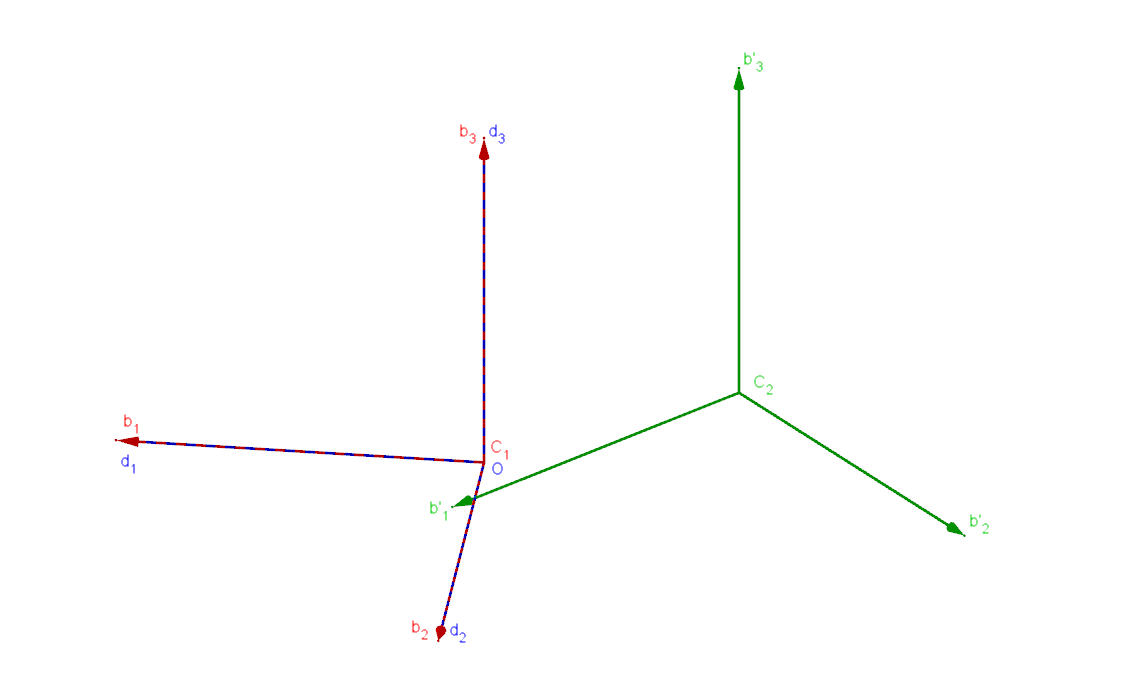
\includegraphics[width=1.\linewidth]{images/GrafikHomographieDifferentC.png}
%	\captionof{figure}{Weltkoordinatensystem $(O,\delta)$ mit $\delta = [\vec{d_1},\vec{d_1},\vec{d_1},O]$ und Kamerakoordinatensysteme $\beta= [\vec{b_1},\vec{b_2},\vec{b_3},C]$ und $(C',\beta')$ mit $\beta'= [\vec{b'_1},\vec{b'_2},\vec{b'_3},C']$ .}
%\end{minipage}\\ \\
%
%Mit $C'$ wird der Ursprung des Koordinatensystems von Kamera zwei bezeichnet. Als Objekte in der Ebene im $\mathbb{R}^3$-Raum, werden die selben Punkt $A_\delta,B_\delta,C_\delta,D_\delta$ und $E_\delta$ wie im vorherigen Beispiel verwendet.\\
%
%\begin{gather}
%	A_\delta=\begin{pmatrix}
%		0\\0\\2\\1
%	\end{pmatrix}, 
%	B_\delta=
%	\begin{pmatrix}
%		1\\0\\2\\1
%	\end{pmatrix},
%	C_\delta=
%	\begin{pmatrix}
%		1\\1\\2\\1
%	\end{pmatrix},
%	D_\delta=
%	\begin{pmatrix}
%		0\\1\\2\\1
%	\end{pmatrix},
%	E_\delta=
%	\begin{pmatrix}
%		\frac{1}{2}\\\frac{1}{2}\\2\\1
%	\end{pmatrix}
%\end{gather}\\
%
%Punkt $E_\delta$ bildet den Mittelpunkt des Quadrates und wird als Drehpunkt gewählt und mit $\textit{PivotPoint}$ bezeichnet. Als nächstes wird Matrix $T$ aus drei Transformationsmatrizen zusammengestellt. Diese Matrix verschiebt das Projektionszentrum von $C'$ an den gewünschten Ort im Weltkoordinatensystem. Bezeichnet werden die drei Matrizen mit $T_1, T_2$ und $T_3$. $T_1$ beinhaltet die Verschiebung von des Ursprungs von Kamera eins zum $\textit{PivotPoint}$, $T_2$ bildet die Rotationsmatrize, welche den Verschobenen Punkt um die gewünschten $45^\circ$ dreht. Die letzte Matrize $T_3$ beinhaltet wieder eine Translation, welche den Punkt vom $\textit{PivotPoint}$ zurück verschiebt. 
%
%\begin{gather}
%	T_1 = \begin{bmatrix}
%		1&0&0&-\textit{PivotPoint}_x\\
%		0&1&0&-\textit{PivotPoint}_y\\
%		0&0&1&-\textit{PivotPoint}_z\\
%		0&0&0&1
%	\end{bmatrix} = 
%	\begin{bmatrix}
%		1&0&0&-\frac{1}{2}\\
%		0&1&0&-\frac{1}{2}\\
%		0&0&1&-2\\
%		0&0&0&1
%	\end{bmatrix}\\
%	T_2 = \begin{bmatrix}
%		\cos(45^\circ)&0&\sin(45^\circ)&0\\
%		0&1&0&0\\
%		-\sin(45^\circ)&0&\cos(45^\circ)&0\\
%		0&0&0&1
%	\end{bmatrix}=
%	\begin{bmatrix}
%		\frac{1}{\sqrt{2}}&0&\frac{1}{\sqrt{2}}&0\\
%		0&1&0&0\\
%		-\frac{1}{\sqrt{2}}&0&\frac{1}{\sqrt{2}}&0\\
%		0&0&0&1
%	\end{bmatrix}\\
%	T_3 = 
%	\begin{bmatrix}
%		1&0&0&\textit{PivotPoint}_x\\
%		0&1&0&\textit{PivotPoint}_y\\
%		0&0&1&\textit{PivotPoint}_z\\
%		0&0&0&1
%	\end{bmatrix} = 
%	\begin{bmatrix}
%		1&0&0&\frac{1}{2}\\
%		0&1&0&\frac{1}{2}\\
%		0&0&1&2\\
%		0&0&0&1
%	\end{bmatrix}\\
%	T= 
%	T_3 \cdot T_2 \cdot T_1
%	= 
%	\begin{bmatrix}
%		\frac{1}{\sqrt{2}}&0&\frac{1}{\sqrt{2}}&-1.26777\\
%		0&1&0&0\\
%		-\frac{1}{\sqrt{2}}&0&\frac{1}{\sqrt{2}}&0.93934\\
%		0&0&0&1
%	\end{bmatrix}\\
%	C'_\delta = T \cdot C_\delta
%	= 	
%	\begin{bmatrix}
%		\frac{1}{\sqrt{2}}&0&\frac{1}{\sqrt{2}}&-1.26777\\
%		0&1&0&0\\
%		-\frac{1}{\sqrt{2}}&0&\frac{1}{\sqrt{2}}&0.93934\\
%		0&0&0&1
%	\end{bmatrix} \cdot 
%	\begin{bmatrix}
%		0\\0\\0\\1
%	\end{bmatrix}
%	=
%	\begin{bmatrix}
%		-1.27\\0\\0.94\\1
%	\end{bmatrix}	
%\end{gather} 
%
%Der Ursprung des Koordinatensystems von Kamera zwei befindet sich, angegeben in Weltkoordinaten, bei $C'_\delta =\begin{bmatrix}-1.26777&0&0.93934&1\end{bmatrix}^T$. Da nun die $C'_\delta$ bekannt ist, können die 3D-Objektpunkte in das Kamerakoordinatensystem von Kamera zwei transformiert werden. Hierzu wird die Matrix $R'$ aufgestellt.
%
%\begin{gather}
%	R' = \begin{bmatrix}
%		&&&\\
%		&[T_2]^{-1}&& -[T_2]^{-1} \cdot V\\
%		&&&\\
%		0&0&0&1\\
%	\end{bmatrix}
%\end{gather}
%
%aufgestellt werden. $V$ ist der Translationsvektor welcher den Wert von $C'_\delta$ bekommt. Da es sich wieder um kartesische Koordinatensysteme handelt gilt wieder $[T_2]^{-1}$ = $[T_2]^{T}$.
%
%\begin{gather}
%	-[T_2]^{T}\cdot C'_\delta = 
%	\begin{pmatrix}
%		\frac{1}{\sqrt{2}}&0&-\frac{1}{\sqrt{2}}\\
%		0&1&0\\
%		\frac{1}{\sqrt{2}}&0&\frac{1}{\sqrt{2}}
%	\end{pmatrix}
%	\cdot
%	\begin{pmatrix}
%		-1.27\\0\\0.94
%	\end{pmatrix}
%	=
%	\begin{pmatrix}
%		1.56\\0\\0.23
%	\end{pmatrix}
%\end{gather}
%
%Für die Transformationsmatrizen $R$ und $R'$ gilt dann jeweils:
%
%\begin{gather}
%	R = 
%	\begin{bmatrix}
%		1&0&0&0\\
%		0&1&0&0\\
%		0&0&1&0\\
%		0&0&0&1
%	\end{bmatrix}\\	
%	R'=
%	\begin{bmatrix}
%		\frac{1}{\sqrt{2}}&0&-\frac{1}{\sqrt{2}}&1.56\\
%		0&1&0&0\\
%		\frac{1}{\sqrt{2}}&0&\frac{1}{\sqrt{2}}&0.23\\
%		0&0&0&1
%	\end{bmatrix}
%\end{gather}\\
%
%Nachdem $R$ und $R'$ bestimmt sind,  müssen die Punkte in Weltkoordinaten noch in die entsprechenden Kamerakoordinatensysteme und mit den Projektionsmatrizen $K$ und $K'$ in deren Bildkoordinatensysteme transformiert werden. Es gilt wieder wie im Beispiel zuvor, dass $K = K'$ ist.
%
%\begin{gather}
%	\leftidx{_{K_{c1}}}{\begin{bmatrix}
%			\pi
%	\end{bmatrix}}{_{K_{c1}}}
%	=		\leftidx{_{K_{c2}}}{\begin{bmatrix}
%			\pi
%	\end{bmatrix}}{_{K_{c2}}}
%	=
%	\begin{pmatrix}
%		\zeta&0&0&0\\
%		0&\zeta&0&0\\
%		0&0&\zeta&0\\
%		0&0&1&0
%	\end{pmatrix}=
%	\begin{pmatrix}
%		-1&0&0&0\\
%		0&-1&0&0\\
%		0&0&-1&0\\
%		0&0&1&0
%	\end{pmatrix}
%\end{gather}
%
%Es entstehen die folgenden beiden Punktematrizen $pC$ für Kamera eins und $pC'$ für Kamera zwei. Die Koordinaten der jeweiligen Punkte $ pC = [A_\tau \;B_\tau\;C_\tau\;D_\tau\;E_\tau$] und $pC' =[A_{\tau'}\;B_{\tau'}\;C_{\tau'}\;D_{\tau'}\;E_{\tau'}]$ aus Sicht der beiden Kameras befinden sich der Reihe nach in den Spalten der Punktematrix.
%
%\begin{gather}
%	pC = 
%	\begin{bmatrix}
%		0&\frac{1}{2}&\frac{1}{2}&0&\frac{1}{4}\\
%		0&0&\frac{1}{2}&\frac{1}{2}&\frac{1}{4}\\
%		1&1&1&1&1
%	\end{bmatrix}\\
%	pC'=
%	\begin{bmatrix}
%		0.09&0.36&0.36&0.09&\frac{1}{4}\\
%		0&0&0.42&0.61&\frac{1}{4}\\
%		1&1&1&1&1
%	\end{bmatrix}\\
%\end{gather}
%
%Die Homographiematrix wird durch aufstellen der Koeffizientenmatrix und anschließendes Bestimmen von $H \cdot x = 0$ oder durch findes desjenigen Vektors $\vec{x}$ für den $||H\cdot x||$ minimal wird. Da es sich auch hier nicht um einen überbestimmten Fall handelt, kann die homographiematrix entweder durch die Bestimmung des Kerns oder durch anwenden der Singulärwertszerlegung $SVD$, gewonnen werden. Die resultierende Homographiematrix sieht folgendermaßen aus.
%
%\begin{gather}
%	H = \begin{bmatrix}
%		0.43&0&0.43\\
%		0&0.6&0\\
%		0.4&0&0.5
%	\end{bmatrix}
%\end{gather}
%
%Wird $H$ auf die Punkte $pC$ angewandt, so liefert das Ergebnis die Punkte von $pC'$ und wird die Inverse $H^{-^1}$ auf die Punkte $pC'$ angewandt, so erhält man die Punkte von $pC$. Somit wurde bewiesen, dass Homographiematrizen immer zur Transformation von Punkte genutzt werden können, solange sich diese Punkte auf einer Ebene im Raum befinden. Die Definition der Homographie sagt aus, dass sowohl Tranlationen und Rotationen in der Homographiematrix vorkommen dürfen \cite{Roser} \cite{Peiffer}. Die Drehung um einen Drehpunkt ist nicht weiter als die Hintereinaderschaltung verschiedener Tranformationsmarizen. Das wichtigste Kriterium welches erfüllt sein muss, damit Homographien angewendet werden können ist, dass die Abbildungen der Punkte in allen Kameras auf einer Ebene sich befinden müssen.\cite{Elements}.
%
%In der Abbildung \ref{fig:DrehungDrehpunkt} ist ein grüner Punkt zu sehen welcher sich in Gegensatz zu den anderen Punkte nicht auf der selben Ebene befindet. Dieser Punkt lässt sich nicht mit der errechneten Homographiematrix ineinander überführen. Mit Hilfe von Homographien, können die Positionen und Orientierung der jeweiligen Kameras zueinander ermittelt werden, jedoch nur wenn sich die Szenepunkte auf einer Ebene befinden. Ein Beispiel hierfür wäre zum beispiel die Aufnahme einer Gebäudefassade aus unterschiedlichen Kamerawinkeln und Positionen\cite{Elements}. Für eine Szenenrekonstruktion einer kompletten 3D-Szene reichen pure Homographien nicht aus, hierfür muss sich der geometrischen Eigenschaften der Epipolargeometrie bedient werden. 
%
